% Options for packages loaded elsewhere
\PassOptionsToPackage{unicode}{hyperref}
\PassOptionsToPackage{hyphens}{url}
%
% Current TDSC draft.
\documentclass[journal]{IEEEtran}
\usepackage{amsmath,amssymb}
\usepackage{lmodern}
\usepackage{iftex}
\ifPDFTeX
  \usepackage[T1]{fontenc}
  \usepackage[utf8]{inputenc}
  \usepackage{textcomp} % provide euro and other symbols
\else % if luatex or xetex
  \usepackage{unicode-math}
  \defaultfontfeatures{Scale=MatchLowercase}
  \defaultfontfeatures[\rmfamily]{Ligatures=TeX,Scale=1}
\fi
% Use upquote if available, for straight quotes in verbatim environments
\IfFileExists{upquote.sty}{\usepackage{upquote}}{}
\IfFileExists{microtype.sty}{% use microtype if available
  \usepackage[]{microtype}
  \UseMicrotypeSet[protrusion]{basicmath} % disable protrusion for tt fonts
}{}
% IEEEtran defines paragraph indentation and spacing; avoid Pandoc's
% parskip defaults because they waste double-column page budget.
\usepackage{xcolor}
\IfFileExists{xurl.sty}{\usepackage{xurl}}{} % add URL line breaks if available
\IfFileExists{bookmark.sty}{\usepackage{bookmark}}{\usepackage{hyperref}}
\hypersetup{
  pdftitle={SessionBound: Database-Enforced Task-Bound Sessions for Enterprise AI Agents},
  pdfauthor={Minmin Wu},
  pdfkeywords={AI agents, access control, database security, dependable computing, secure computing, authorization, SQL security, data governance, auditability},
  hidelinks,
  pdfcreator={LaTeX with IEEEtran}}
\urlstyle{same} % disable monospaced font for URLs
\usepackage{color}
\usepackage{fancyvrb}
\newcommand{\VerbBar}{|}
\newcommand{\VERB}{\Verb[commandchars=\\\{\}]}
\DefineVerbatimEnvironment{Highlighting}{Verbatim}{
  commandchars=\\\{\},
  fontsize=\scriptsize
}
% Add ',fontsize=\small' for more characters per line
\newenvironment{Shaded}{}{}
\newcommand{\AlertTok}[1]{\textcolor[rgb]{1.00,0.00,0.00}{#1}}
\newcommand{\AnnotationTok}[1]{\textcolor[rgb]{0.38,0.63,0.69}{#1}}
\newcommand{\AttributeTok}[1]{\textcolor[rgb]{0.49,0.56,0.16}{#1}}
\newcommand{\BaseNTok}[1]{\textcolor[rgb]{0.25,0.63,0.44}{#1}}
\newcommand{\BuiltInTok}[1]{#1}
\newcommand{\CharTok}[1]{\textcolor[rgb]{0.25,0.44,0.63}{#1}}
\newcommand{\CommentTok}[1]{\textcolor[rgb]{0.38,0.63,0.69}{#1}}
\newcommand{\CommentVarTok}[1]{\textcolor[rgb]{0.38,0.63,0.69}{#1}}
\newcommand{\ConstantTok}[1]{\textcolor[rgb]{0.53,0.00,0.00}{#1}}
\newcommand{\ControlFlowTok}[1]{\textcolor[rgb]{0.00,0.44,0.13}{#1}}
\newcommand{\DataTypeTok}[1]{\textcolor[rgb]{0.56,0.13,0.00}{#1}}
\newcommand{\DecValTok}[1]{\textcolor[rgb]{0.25,0.63,0.44}{#1}}
\newcommand{\DocumentationTok}[1]{\textcolor[rgb]{0.73,0.13,0.13}{#1}}
\newcommand{\ErrorTok}[1]{\textcolor[rgb]{1.00,0.00,0.00}{#1}}
\newcommand{\ExtensionTok}[1]{#1}
\newcommand{\FloatTok}[1]{\textcolor[rgb]{0.25,0.63,0.44}{#1}}
\newcommand{\FunctionTok}[1]{\textcolor[rgb]{0.02,0.16,0.49}{#1}}
\newcommand{\ImportTok}[1]{#1}
\newcommand{\InformationTok}[1]{\textcolor[rgb]{0.38,0.63,0.69}{#1}}
\newcommand{\KeywordTok}[1]{\textcolor[rgb]{0.00,0.44,0.13}{#1}}
\newcommand{\NormalTok}[1]{#1}
\newcommand{\OperatorTok}[1]{\textcolor[rgb]{0.40,0.40,0.40}{#1}}
\newcommand{\OtherTok}[1]{\textcolor[rgb]{0.00,0.44,0.13}{#1}}
\newcommand{\PreprocessorTok}[1]{\textcolor[rgb]{0.74,0.48,0.00}{#1}}
\newcommand{\RegionMarkerTok}[1]{#1}
\newcommand{\SpecialCharTok}[1]{\textcolor[rgb]{0.25,0.44,0.63}{#1}}
\newcommand{\SpecialStringTok}[1]{\textcolor[rgb]{0.73,0.40,0.53}{#1}}
\newcommand{\StringTok}[1]{\textcolor[rgb]{0.25,0.44,0.63}{#1}}
\newcommand{\VariableTok}[1]{\textcolor[rgb]{0.10,0.09,0.49}{#1}}
\newcommand{\VerbatimStringTok}[1]{\textcolor[rgb]{0.25,0.44,0.63}{#1}}
\newcommand{\WarningTok}[1]{\textcolor[rgb]{0.38,0.63,0.69}{#1}}
\usepackage{longtable,booktabs,array}
\usepackage{tikz}
\usetikzlibrary{arrows.meta,positioning,shapes.geometric}
\newcounter{algorithm}
\usepackage{calc} % for calculating minipage widths
% Correct order of tables after \paragraph or \subparagraph
\usepackage{etoolbox}
\makeatletter
\patchcmd\longtable{\par}{\if@noskipsec\mbox{}\fi\par}{}{}
\makeatother
% Allow footnotes in longtable head/foot
\IfFileExists{footnotehyper.sty}{\usepackage{footnotehyper}}{\usepackage{footnote}}
\makesavenoteenv{longtable}
\setlength{\emergencystretch}{3em} % prevent overfull lines
\providecommand{\tightlist}{%
  \setlength{\itemsep}{0pt}\setlength{\parskip}{0pt}}
\setcounter{secnumdepth}{3}
\ifLuaTeX
  \usepackage{selnolig}  % disable illegal ligatures
\fi

\title{SessionBound: Database-Enforced Task-Bound Sessions for
Enterprise AI Agents}
\author{Minmin~Wu\\
China Telecom Global Limited\\
\href{mailto:wuminmin@chinatelecomglobal.com}{wuminmin@chinatelecomglobal.com}}

\begin{document}

\maketitle

\begin{abstract}

Enterprise AI agents can write useful exploratory SQL for audit,
compliance, and operational analysis, but raw database access is
over-privileged and fixed SaaS screens are too rigid for temporary
business tasks. This paper presents SessionBound, a database-enforced
task-bound session model for enterprise AI agents. A control plane turns
an approved task into a signed token carrying task scope, safe views,
denied fields, TTL, operation policy, budgets, and policy-version claims.
The PostgreSQL runtime, SessionBoundDB, binds the token to a short-lived
credential and enforces the approved boundary through safe-view
resolution, read-only SQL policy, disclosure accounting,
minimum-group aggregate protection, schema-drift checks, and receipts.

SessionBoundDB implements an accounting-complete wrapper reference path
and a native PostgreSQL hook/executor hardening path. The evaluation
validates 24 canonical scenarios and a 140-case adversarial SQL suite,
blocking 126 boundary-violation cases while allowing and accounting for
14 safe-view analytical cases. A stronger
RLS+safe-view+short-credential+audit baseline shows that conventional
database controls cover
important pieces but do not provide task-token binding, cumulative
disclosure budgets, safe-view drift invalidation, or receipt chains. On
the default seed, full SessionBound has 128.4--136.1 ms p50 latency in
the wrapper path after statement-start owner validation. Diagnostic
scale benchmarks show that structural guarding is sub-millisecond, while
unoptimized result accounting becomes the bottleneck for larger
detail-release stress settings. These results support SessionBound as a
task-session contract for database-enforced AI-agent governance, while
identifying executor-level accounting optimization as future work.
\end{abstract}

\begin{IEEEkeywords}
AI agents, access control, database security, dependable computing,
secure computing, authorization, SQL security, data governance,
auditability.
\end{IEEEkeywords}

\hypertarget{introduction}{%
\section{Introduction}\label{introduction}}

AI agents change how enterprise users interact with data. A user no
longer needs to know which report exists, which dashboard to open, or
which API endpoint to call. Instead, the user can ask an agent:

\begin{quote}
Analyze June 2026 travel reimbursements for the Sales department. Find
unusual merchants, repeated claims, employee-level monthly totals, and
claims near approval thresholds. Exclude salary and bank data.
\end{quote}

This is exactly the kind of task agents are good at: temporary,
exploratory, cross-table, and under-specified. It is also exactly the
kind of task traditional enterprise software handles poorly. Building a
permanent SaaS page or API for every low-frequency internal analysis
task is expensive. Giving the agent raw database access is unsafe.
Relying on prompts is not a security boundary. Relying on the
application layer alone becomes fragile when SQL is generated
dynamically.

Existing systems cover important pieces: delegated identity and OAuth
scopes~\cite{rfc6749,south2025authenticateddelegation}, task-scoped tool
authorization~\cite{sharma2026pauth}, data-product
governance~\cite{tonnarelli2026dataproductmcp,mcp2025specification},
database-native policy enforcement~\cite{postgresql2026rowsecurity,oracle2026vpd,oracle2026deepdatasecuritydocs},
purpose-based database controls~\cite{agrawal2002hippocratic,byun2008purpose},
query auditing and inference control~\cite{kleinberg2000auditing,nabar2006robustness},
database proxies/reference monitors, and large-scale relationship authorization
~\cite{pang2019zanzibar}.
They do not, by themselves, turn one approved analytical task into a
temporary SQL session with safe views, denied fields, budgets, and
receipts. We therefore evaluate both a conventional RLS/safe-view/short-login
baseline and a functionally equivalent composition that adds an external
signature/credential PEP, tuple budgeting, and audit; the latter is equivalent
only while every request traverses the external reference monitor. That is the
gap SessionBound addresses inside the database boundary.

This paper argues for the following principle: business users approve
tasks, not database policies. Agents generate SQL, but databases enforce
the approved boundary. This paper frames the problem as a
database-enforced authorization boundary for enterprise AI agents,
rather than as an agent-planning or multi-agent coordination problem.
SessionBound treats an approved enterprise task as the unit of database
execution, rather than treating identity, role, relation, or individual
query as the sole authorization unit. The agent can try. The database
decides.

SessionBound separates a task control plane that approves and signs
structured claims, an agent execution layer that proposes SQL, and a
database runtime that deterministically enforces safe views, scope,
denied fields, operation limits, budgets, and receipts.

This makes SessionBound a contract layer between enterprise approval and
agentic database execution. The control plane records what the
organization approved; the runtime enforces how that approval may be
spent through SQL. This contract is not a database policy written by a
DBA, nor a natural-language instruction interpreted by an LLM. It is a
structured, signed, and accountable representation of an approved
business task that both the agent runtime and the database can interpret
deterministically.

SessionBoundDB is our PostgreSQL-based reference runtime for
SessionBound. It does not ask an LLM whether a query is safe. It does
not depend on the agent correctly interpreting the task. It does not
trust mutable session variables set by the agent. Instead, it validates
a signed task token, exposes only registered safe views, rejects raw
table access and denied fields, tracks query and disclosure budgets, and
records receipts for evaluated allowed executions and bound-runtime
denial decisions.

The novelty is not any single primitive. It is the binding of task
approval, credential identity, safe-view versioning, SQL surface,
cumulative disclosure budget, and receipt semantics into one
database-execution session object: enterprise task approval is compiled
into an execution-time database session contract rather than scattered
across separate credentials, views, policies, and audit logs.

\hypertarget{contributions}{%
\subsection{Contributions}\label{contributions}}

This paper makes five contributions.

\begin{enumerate}
\def\labelenumi{\arabic{enumi}.}
\item
  Task-bound database sessions. We identify the approved enterprise
  task, rather than only identity, role, relation, or query, as the
  stateful authorization object for agentic SQL.
\item
  Signed control-plane contract. Templates, applications, approvals,
  grants, TTLs, budgets, and task tokens become database-consumable
  structured claims rather than natural language.
\item
  Composed session object. Credential-token matching, safe-view
  versioning, exposed-column hashing, disclosure budgets, minimum-group
  policy, and receipts are bound into one session object.
\item
  PostgreSQL prototype with wrapper and native hardening paths.
  We implement an accounting-complete wrapper/API reference path and a
  native PostgreSQL hook/executor path for direct safe-view SQL,
  prepared statements, cursor/\texttt{FETCH}, \texttt{COPY (SELECT)},
  utility checks, and executor-level accounting.
\item
  Evaluation against stronger baselines and attacks. We evaluate
  canonical behavior, adversarial SQL, credential-token binding, drift
  invalidation, a strong RLS+safe-view+short-credential audit baseline,
  ablations, scale behavior, and hook-only structural cost.
\end{enumerate}


\hypertarget{motivation-enterprise-tasks-are-approved-above-the-database}{%
\section{Motivation: Enterprise Tasks Are Approved Above the
Database}\label{motivation-enterprise-tasks-are-approved-above-the-database}}

SessionBound targets temporary enterprise analysis that is too specific
for a permanent application screen and too sensitive for raw database
access: reimbursement audits, vendor-concentration checks, compliance-log
reviews, or operational investigations. These tasks need joins,
aggregation, ranking, drill-down, and follow-up SQL, but the exact query
plan is not known when the task is approved.

For example, a business user may request a June 2026 Sales travel
reimbursement audit that excludes salary, phone, and bank-account
fields, allows 20 SQL attempts and 5,000 result rows, and expires after
30 minutes. A manager or data owner can approve this task without writing RLS
predicates or database grants. A data platform can expose safe views. A
compliance policy can tighten budgets. The agent can then generate SQL
inside the approved boundary, while the database rejects raw tables,
denied fields, unsafe operations, and over-budget attempts.


\hypertarget{threat-model}{%
\section{Threat Model}\label{threat-model}}

SessionBound assumes the upper-layer agent is useful but not trusted.
The agent may be confused, overconfident, prompt-injected, malicious, or
simply wrong. The database boundary must remain meaningful even when the
agent tries the wrong thing.

\hypertarget{trusted-components}{%
\subsection{Trusted components}\label{trusted-components}}

For this prototype, we trust:

\begin{itemize}
\tightlist
\item
  the task control plane that defines templates, evaluates grants,
  records approvals, and signs task tokens;
\item
  the credential broker that issues short-lived database credentials;
\item
  the database runtime that validates tokens and enforces policies;
\item
  the PostgreSQL lock manager on one writable primary, including
  session-level advisory-lock cleanup when a backend exits;
\item
  the cryptographic signing key or signing service used for task tokens;
\item
  the integrity of registered safe views, runtime functions, and
  DB-local append-only audit storage.
\end{itemize}

In production, signing should use a KMS, JWKS, hardware-backed key
service, or enterprise identity infrastructure. The prototype uses a
simpler signing path. Receipt-chain tamper evidence assumes trusted
DB-local append-only storage; DBA-resistant deployments should anchor
chain heads to external WORM storage, SIEM, transparency logs, or
enterprise audit infrastructure.
The global single-active binding guarantee in this prototype is scoped
to one non-split-brain PostgreSQL primary. Database-cluster split brain
and cross-cluster global ownership require external primary fencing and
are not solved by SessionBound's advisory-lock protocol.

The trusted-computing base (TCB) is therefore explicit rather than implicit:
the signer and credential registry, the single-primary PostgreSQL lock and
transaction manager, the \texttt{sessionbound\_guard} hooks, the runtime SQL
functions, the safe-view definitions and registry hashes, and the append-only
receipt store. A safe-view definition is a policy artifact in this TCB; if it
is over-broad, the runtime can only detect a hash/version drift, not infer that
the definition is semantically unsafe. The database-enforced claim is limited
to the reference-monitor interface below and is not a claim about arbitrary
SQL or arbitrary semantic inference.

For the evaluated fragment, the reference monitor accepts one parsed
single-statement \texttt{SELECT} (or the explicitly enumerated
\texttt{COPY (SELECT)} and \texttt{EXPLAIN} utility forms) whose relation OIDs resolve to the token's approved
safe-view registry. It rejects set-operation stacking, recursive CTEs, table
functions, blocked payload aggregation, raw/catalog relations, mutations,
DDL, and session-state utilities. The executor then stages and charges the
complete result before release. The wrapper and native paths implement the
same acceptance predicate and tuple-budget/receipt state transition; their
only operational difference is PL/pgSQL row materialization versus the C
executor tuplestore. This is the scope of the reference-monitor argument,
not a universal PostgreSQL equivalence theorem.

\hypertarget{untrusted-or-partially-trusted-components}{%
\subsection{Untrusted or partially trusted
components}\label{untrusted-or-partially-trusted-components}}

We do not trust:

\begin{itemize}
\tightlist
\item
  the agent's prompt;
\item
  the agent's reasoning;
\item
  the agent's SQL generation;
\item
  the agent's natural-language interpretation of the task;
\item
  user-provided or database-provided text that may contain prompt
  injection;
\item
  ordinary client-controlled session variables;
\item
  application-layer filtering as the final boundary.
\end{itemize}

This is the main difference from designs that require an LLM to infer
the precise intended operation from natural language. SessionBound does
not ask the database to understand the user's natural-language intent.
The database consumes structured claims from a signed token.

\hypertarget{in-scope-threats}{%
\subsection{In-scope threats}\label{in-scope-threats}}

SessionBoundDB is designed to mitigate:

\begin{itemize}
\tightlist
\item
  Sensitive field access: attempts to read salary, bank
  account, phone, identity number, credentials, or private notes.
\item
  Raw table access: attempts to bypass safe views and query
  application schemas directly.
\item
  Scope escape: attempts to read other tenants, months,
  departments, projects, or users.
\item
  Unauthorized mutations: write, DDL, or other high-impact operations
  outside controlled commands.
\item
  Prompt injection effects: data or user text instructs the
  agent to ignore policy or reveal secrets.
\item
  Budget evasion: repeated queries, pagination, or alternate
  SQL forms attempt to disclose more detail rows than the task allows.
\item
  Credential-token mismatch: attempts to combine one runtime
  credential with another task token.
\end{itemize}

\hypertarget{out-of-scope}{%
\subsection{Out of scope}\label{out-of-scope}}

The prototype does not solve:

\begin{itemize}
\tightlist
\item
  malicious DBAs, storage administrators, or compromised database hosts;
\item
  compromised signing or audit infrastructure;
\item
  side-channel attacks;
\item
  complete formal verification of SQL equivalence;
\item
  a production-grade formal SQL safety proof across all PostgreSQL
  features;
\item
  cross-database federation;
\item
  full differential privacy for statistical releases;
\item
  arbitrary semantic inference across all allowed query answers.
\end{itemize}

SessionBound reduces and accounts for what an agent can discover. It
does not claim to eliminate all inference and does not provide
differential privacy.


\hypertarget{sessionbound-model}{%
\section{SessionBound Model}\label{sessionbound-model}}

SessionBound has two major layers: a task control plane and a database
runtime. The control plane turns enterprise task approval into a signed
task token; the database runtime binds that token to a short-lived
credential and enforces safe views, denied fields, budgets, aggregate
policy, drift checks, and receipts inside the database session.

\begin{figure}[!t]
\centering
\scriptsize
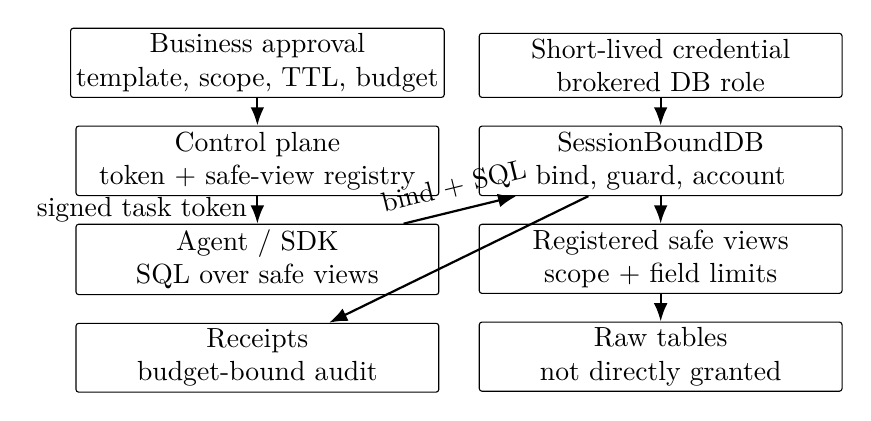
\begin{tikzpicture}[
  node distance=3.5mm,
  box/.style={draw, rounded corners=1pt, align=center, inner sep=2pt, minimum height=6mm},
  arr/.style={-Latex, thick}
]
\node[box, minimum width=0.38\linewidth] (approval) {Business approval\\template, scope, TTL, budget};
\node[box, below=of approval, minimum width=0.38\linewidth] (control) {Control plane\\token + safe-view registry};
\node[box, below=of control, minimum width=0.38\linewidth] (agent) {Agent / SDK\\SQL over safe views};
\node[box, right=5mm of control, minimum width=0.38\linewidth] (db) {SessionBoundDB\\bind, guard, account};
\node[box, above=of db, minimum width=0.38\linewidth] (cred) {Short-lived credential\\brokered DB role};
\node[box, below=of db, minimum width=0.38\linewidth] (views) {Registered safe views\\scope + field limits};
\node[box, below=of views, minimum width=0.38\linewidth] (raw) {Raw tables\\not directly granted};
\node[box, below=of agent, minimum width=0.38\linewidth] (audit) {Receipts\\budget-bound audit};
\draw[arr] (approval) -- (control);
\draw[arr] (control) -- node[left] {signed task token} (agent);
\draw[arr] (cred) -- (db);
\draw[arr] (agent) -- node[above, sloped] {bind + SQL} (db);
\draw[arr] (db) -- (views);
\draw[arr] (views) -- (raw);
\draw[arr] (db) -- (audit);
\end{tikzpicture}
\caption{SessionBound architecture. The approved enterprise task becomes
a signed database-session contract; agents can attempt SQL, but the
database runtime enforces the bound task state.}
\label{fig:architecture}
\end{figure}

\noindent\textbf{Task-bound session state machine.}
SessionBound treats an approved enterprise task as a stateful database
authorization object. A session state is
\(S=\langle A,C,T,V,L,B,R\rangle\), where \(A\) is the approved task,
\(C\) is the brokered credential, \(T\) is the signed token, \(V\) is the
safe-view registry snapshot, \(L\) is the permitted SQL surface, \(B\) is
the remaining budget vector, and \(R\) is the receipt chain. Transitions
include \(\mathsf{issue}\) (approval to token), \(\mathsf{bind}\) (token
and credential to active database state), \(\mathsf{attempt}\) (SQL
shape and safe-view resolution), \(\mathsf{release}\) (budgeted allowed
result), \(\mathsf{deny}\) (receipt-bearing rejection), and
\(\mathsf{expire/revoke/drift}\) (fail-closed invalidation). The
contribution is this state machine around a database session, not a new
identity credential, view mechanism, or audit log in isolation.

\hypertarget{template-application-approval-and-token}{%
\subsection{Template, application, approval, and token}\label{template-application-approval-and-token}}

A task template is defined by a data platform or application team, not by
the agent. It names the task type, purpose, allowed safe views, denied
columns, required scope fields, allowed operations, default TTL, budget
vector, and aggregate policy. A task application instantiates that
template with a requester, actor, concrete scope, and business reason. A
task approval decides whether that scoped task should exist; it may be
automatic, role-based, or manual, but it does not require the approver to
write SQL policies.

The approved task becomes a signed token consumed by the database
runtime. In the prototype, the token binds the task id and type,
delegator, actor, credential id, tenant and row scope, allowed views,
denied columns, permitted operations, query and disclosure budgets,
minimum-group aggregate policy, safe-view registry version, policy
version, view-definition and exposed-column hashes, audience, expiry,
and nonce. The token is structured authorization data, not a natural
language prompt.

\hypertarget{budgeted-database-session}{%
\subsection{Budgeted database
session}\label{budgeted-database-session}}

A budgeted database session is a database session bound to one active
task token. The session may issue open-ended SQL, but every attempt is
checked against the token, safe view registry, operation policy, and
remaining budget.

In the current prototype, a direct database connection may issue native
\texttt{SELECT} over approved safe views after binding a signed task
token. The PostgreSQL extension checks SQL shape and safe-view OIDs,
then executor accounting charges every released result tuple (the
legacy \texttt{unique\_expense\_rows} column is a conservative tuple
counter) before tuples are released. Projection aliases, joins, and
aggregate output cannot avoid the output-row charge; hidden source
entities are not claimed to be counted. The same path covers SDK
\texttt{query(sql)}, bound direct \texttt{SELECT}, prepared statements,
cursor/\texttt{FETCH}, \texttt{COPY (SELECT)}, and non-\texttt{ANALYZE}
\texttt{EXPLAIN}. Raw table \texttt{SELECT} remains ungranted; schema
resolution is allowed only so the hook can fail closed and emit receipts.
Pooled connections can rebind only with a fresh valid token and can call
\texttt{unbind\_task()} at check-in.


\hypertarget{control-plane-templates-applications-approvals-and-budgets}{%
\section{Control Plane: Templates, Applications, Approvals, and
Budgets}\label{control-plane-templates-applications-approvals-and-budgets}}

The control plane is the enterprise layer that converts business
approval into database-enforceable structure. A data owner approves a
task such as ``Alice may run a June 2026 Sales travel reimbursement
review, excluding salary, bank-account, and phone fields, under a
30-minute TTL and bounded disclosure budget.'' The approver should not
need to author \texttt{CREATE POLICY}, \texttt{ALTER ROLE}, or
\texttt{GRANT} statements.

Roles grant eligibility to request task templates, not broad database
access. For example, a finance reviewer may request finance-review
tasks and a department manager may request department-scoped analysis
tasks, but the database ultimately sees a concrete signed task token:
actor \(X\) may analyze June 2026 Sales reimbursements through approved
views under budget \(Y\). Budget assignment remains a control-plane
decision based on role, data classification, task purpose, and approval
route; the database runtime enforces the resulting budget.


\hypertarget{sessionbounddb-runtime}{%
\section{SessionBoundDB Runtime}\label{sessionbounddb-runtime}}

SessionBoundDB is the PostgreSQL-based database runtime for
SessionBound.

\hypertarget{session-binding-and-credential-token-binding}{%
\subsection{Session binding and credential-token
binding}\label{session-binding-and-credential-token-binding}}

The runtime begins with two objects:

\begin{enumerate}
\def\labelenumi{\arabic{enumi}.}
\tightlist
\item
  a short-lived database credential issued by the credential broker;
\item
  a signed task token issued by the control plane.
\end{enumerate}

The credential authenticates the runtime connection. The task token
authorizes the work.

At \texttt{bind\_task}, the runtime checks:

\begin{itemize}
\tightlist
\item
  the task token signature is valid;
\item
  the task token is unexpired and not revoked;
\item
  the credential is unexpired and not revoked;
\item
  the token \texttt{credential\_id} matches the current session
  credential;
\item
  the token \texttt{actor} matches the credential actor;
\item
  the session login role matches the broker-issued database user;
\item
  the token audience is \texttt{sessionbounddb};
\item
  this backend has no other active binding;
\item
  no other PostgreSQL backend owns the same
  \((\texttt{task\_id},\texttt{token\_digest},\texttt{credential\_id})\)
  binding key.
\end{itemize}

The last check is global within one writable PostgreSQL primary.
\texttt{bind\_task} derives a stable 64-bit session advisory-lock key
from the exact binding key using a fixed SHA-256 prefix, obtains it with
non-blocking \texttt{pg\_try\_advisory\_lock}, claims a protected active
row, allocates a fresh \texttt{binding\_id} and monotonic
\texttt{fence\_token}, and only then installs backend-local trusted
state. The active row is protected by uniqueness on
\((\texttt{task\_id},\texttt{token\_digest},\texttt{credential\_id})\)
and on \texttt{binding\_id}; budget, receipt, cleanup, and unbind
mutations carry the current \texttt{binding\_id}/\texttt{fence\_token}.
Hash collisions in the advisory-lock key can cause conservative
rejection but cannot grant two owners the same exclusive lock.

A production implementation should make a stolen credential without a
matching token insufficient, and a stolen token without the matching
credential insufficient. Credential-token binding is intended to reduce
cross-task credential misuse.

PostgreSQL nuance: inside \texttt{SECURITY\ DEFINER} functions,
\texttt{current\_user} may refer to the function owner. Therefore, a
production implementation should use \texttt{session\_user} and/or an
explicit credential registry mapping rather than relying on
\texttt{current\_user} alone. The measured prototype validates token
signatures, token expiration, revoked task state, credential-id-to-token
matching, actor matching, audience validation, cross-credential token
replay rejection, and same-session rebind rejection in the tested
prototype path; Section~\ref{evaluation} reports those tests explicitly.
Production deployments still require hardened credential brokerage, key
management, and audit-retention integration outside this demo.

\hypertarget{safe-views-as-the-query-surface}{%
\subsection{Safe views as the query
surface}\label{safe-views-as-the-query-surface}}

Agents do not query raw application tables. They query registered safe
views. Safe views expose business objects, not internal schemas. This is
complementary to database-native mechanisms such as PostgreSQL
row-level security policies, which provide row filtering at the database
layer~\cite{postgresql2026rowsecurity}.

Safe views are trusted policy artifacts reviewed by data platform, DBA,
and security teams, not agents or ordinary business users. Agents should
not have catalog privileges exposing sensitive view definitions.
Migrations require review, hash/version updates, and task reapproval; a
leaky safe view is a governance failure outside the runtime SQL guard.

Example safe views:

\begin{verbatim}
expenses
employees
departments
approval_events
ledger_entries
\end{verbatim}

A safe view may:

\begin{itemize}
\tightlist
\item
  join raw tables into business objects;
\item
  remove sensitive fields;
\item
  apply tenant, department, month, or project scope;
\item
  expose workflow hints;
\item
  include stable business identifiers for budget accounting.
\end{itemize}

Safe views are not a complete inference-control solution. They reduce
the discoverable surface and make it governable.

\hypertarget{operation-policy}{%
\subsection{Operation policy}\label{operation-policy}}

Native PostgreSQL \texttt{SELECT} is the database accounting entrypoint
for read-only analytical SQL. The agent-facing SDK exposes this as
\texttt{query(sql)}: the agent supplies ordinary SQL over approved
safe-view names, and PostgreSQL hook and executor paths enforce the task
boundary, debit query and disclosure budgets, and emit receipts.
\texttt{taskbound.run(sql)} remains as a compatibility wrapper. High-value
writes should use controlled commands or stored procedures. The runtime
rejects mutations, DDL, unsafe utility commands, raw schema access,
denied fields, and blocked schemas.

\hypertarget{query-decision-pipeline}{%
\subsection{Query decision
pipeline}\label{query-decision-pipeline}}

At runtime, every SQL attempt follows the deterministic decision
procedure in Algorithm~\ref{alg:sql-decision-pipeline}.

\begin{center}
\refstepcounter{algorithm}\label{alg:sql-decision-pipeline}
\begin{minipage}{0.9\linewidth}
Algorithm \thealgorithm. SQL decision pipeline for SessionBoundDB

Input: SQL attempt and bound database session state.

Output: Allowed result with receipt, or denial receipt.

\begin{enumerate}
\item Require ownership of the global active binding and validate
  \texttt{binding\_id}/\texttt{fence\_token}.
\item Validate the signed task token and its TTL.
\item Resolve all referenced relations against registered safe views.
\item Reject denied fields and blocked schemas.
\item Enforce row scope predicates for the bound task.
\item Reject disallowed operation types, including mutations, DDL, and
unsafe utility commands.
\item Reserve query budget before execution.
\item Execute only after the structural checks pass.
\item Account every candidate output tuple before wrapper release or
before native forwarding; aliases and aggregates use the same conservative
output-tuple charge.
\item Emit an allow receipt for a covered release; otherwise reject the
attempt and emit a denial receipt.
\end{enumerate}
\end{minipage}
\end{center}

The runtime does not ask an LLM whether a query is safe.

\begin{figure}[!t]
\centering
\scriptsize
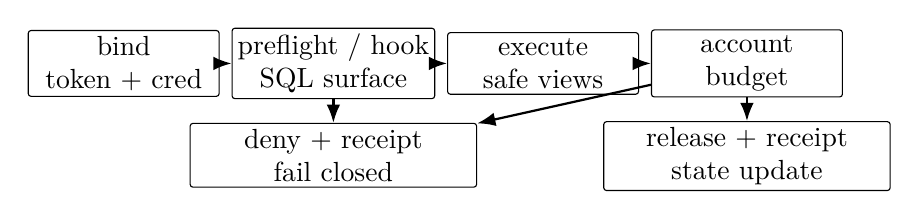
\begin{tikzpicture}[
  node distance=3mm,
  box/.style={draw, rounded corners=1pt, align=center, inner sep=2pt, minimum height=6mm},
  arr/.style={-Latex, thick}
]
\node[box, minimum width=0.20\linewidth] (bind) {bind\\token + cred};
\node[box, right=1.5mm of bind, minimum width=0.20\linewidth] (guard) {preflight / hook\\SQL surface};
\node[box, right=1.5mm of guard, minimum width=0.20\linewidth] (exec) {execute\\safe views};
\node[box, right=1.5mm of exec, minimum width=0.20\linewidth] (acct) {account\\budget};
\node[box, below=of guard, minimum width=0.30\linewidth] (deny) {deny + receipt\\fail closed};
\node[box, below=of acct, minimum width=0.30\linewidth] (allow) {release + receipt\\state update};
\draw[arr] (bind) -- (guard);
\draw[arr] (guard) -- (exec);
\draw[arr] (exec) -- (acct);
\draw[arr] (acct) -- (allow);
\draw[arr] (guard) -- (deny);
\draw[arr] (acct) -- (deny);
\end{tikzpicture}
\caption{Bind/query decision pipeline. Both paths stage and account the
candidate result before release; the native path uses a private tuplestore
so an over-budget query releases no prefix.}
\label{fig:bind-query-pipeline}
\end{figure}


\hypertarget{security-invariants}{%
\section{Security Invariants}\label{security-invariants}}

The SessionBoundDB enforcement contract can be described by a state

\begin{equation}
S=\langle T,C,G,V,B,R\rangle,
\end{equation}

where \(T\) is the signed task token, \(C\) is the credential/session
binding, \(G\) is global active-binding ownership over
\((\texttt{task\_id},\texttt{token\_digest},\texttt{credential\_id})\)
including \texttt{binding\_id}, \texttt{fence\_token}, advisory lock,
and backend owner metadata, \(V\) is the safe-view registry and policy
version, \(B\) is the remaining budget vector, and \(R\) is the receipt chain. Each SQL
attempt is evaluated by:

\begin{equation}
\begin{aligned}
decide(q,S) &\rightarrow allow(result,S')\\
            &\quad \mathrm{or}\; deny(reason,receipt,S').
\end{aligned}
\end{equation}

These invariants define the enforcement contract implemented by the
prototype and used to structure the adversarial evaluation. They are not
a formal proof that all semantic inference is impossible.

\begin{itemize}
\tightlist
\item
  I1. No SQL execution occurs without an active task binding.
\item
  I1a. For one exact binding key, at most one PostgreSQL backend may be
  ACTIVE at any time on the same writable primary.
\item
  I2. The bound token must match the session credential, actor,
  audience, expiry, token digest, and revocation state.
\item
  I3. Referenced relations must belong to the approved safe-view
  registry.
\item
  I4. Direct access to denied fields, raw schemas, catalog escape,
  mutation, DDL, and blocked payload aggregation is denied.
\item
  I5. Scope predicates or session-bound claims constrain visible rows.
\item
  I6. Budget state is monotonic: an allowed query consumes budget, or
  the query is denied; all budget and receipt mutations are fenced by
  the current \texttt{binding\_id}/\texttt{fence\_token}.
\item
  I7. Every evaluated allowed execution and every bound-runtime denial
  emits a receipt; connection-level failures before task binding may be
  logged outside the task receipt chain.
\item
  I8. Safe-view registry, policy version, or definition-hash drift
  invalidates the token or requires reapproval.
\item
  I9. Direct small-group aggregate release is denied under the
  configured minimum-group policy.
\end{itemize}

In the prototype, I1--I2 and I8 are checked during
\texttt{taskbound.bind\_task}; I3--I4 are checked by API-layer AST
preflight, the experimental \texttt{sessionbound\_guard} PostgreSQL
hook path, and database permissions; I5 is enforced by safe-view
predicates; I6 is implemented through task execution state; I7 is
implemented through execution and denial receipts after binding; and I9
is implemented by API shape checks plus wrapper/runtime
entity-cardinality checks, with
conservative native shape checks for direct SQL. Production implementations
should harden these structural checks into always-on planner or executor
integration, but the invariant set is independent of that implementation
choice.

\hypertarget{security-guarantees-for-the-prototype-sql-fragment}{%
\subsection{Security Guarantees for the Prototype SQL
Fragment}\label{security-guarantees-for-the-prototype-sql-fragment}}

We state the prototype security contract over a deliberately restricted
SQL fragment. Let \(\mathrm{SELECT}\text{-}F\) denote single-statement,
read-only SQL consisting of \texttt{SELECT}, projection, predicates,
joins, \texttt{GROUP\ BY}/\texttt{HAVING}, ordering and limits,
non-recursive CTEs, and window functions over registered safe-view
names. The fragment excludes stacked statements, DDL, DML,
\texttt{COPY}, \texttt{DO}, \texttt{CALL}, \texttt{CREATE\ FUNCTION},
temporary object creation, recursive CTEs, set-operation stacking,
table functions, raw-schema or catalog references, and high-risk payload
aggregation such as \texttt{json\_agg}, \texttt{jsonb\_agg},
\texttt{array\_agg}, \texttt{string\_agg}, \texttt{xmlagg},
\texttt{row\_to\_json}, \texttt{json\_build\_object}, and
\texttt{jsonb\_build\_object}. The evaluated \texttt{COPY (SELECT)}
support is an engineering extension routed through the same
relation-resolution and executor-accounting path; the propositions below
are stated only for \(\mathrm{SELECT}\text{-}F\).

Let \(\mathrm{Rels}(q)\) be the set of relation identifiers in \(q\)
after database name resolution and before safe-view expansion. Let
\(\mathrm{Views}(T,V)\) be the approved safe views carried by token \(T\)
and validated against registry \(V\). Let \(\mathrm{Cols}_{out}(q)\) be
the direct column references that appear in the output expressions of
\(q\). A state \(S=\langle T,C,V,B,R\rangle\) is well formed when the
token is valid and bound to credential \(C\), the safe-view registry and
policy hashes match the token, the budget vector \(B\) is nonnegative,
and the receipt chain \(R\) verifies. Under these assumptions, the
prototype provides the following direct-reference and accounting
guarantees. These are not guarantees against arbitrary semantic
inference from allowed answers, and they are not differential privacy.

\noindent\textbf{Proposition 1 (Safe-surface confinement).}
For any well-formed state \(S\) and query
\(q \in \mathrm{SELECT}\text{-}F\), if
\(decide(q,S)=allow(result,S')\), then
\(\mathrm{Rels}(q)\subseteq \mathrm{Views}(T,V)\). Consequently, every
raw base relation evaluated during query execution is reached only
through the definition of a registered safe view approved for the task;
the query has no direct reference path to raw tables or catalogs.

\emph{Argument.} The decision pipeline resolves relation identifiers and
checks them against the task's approved safe-view registry before any
result is released. Database permissions deny raw-schema access, while
the AST preflight and hook path reject resolved relation OIDs outside
the approved safe-view set. Therefore any query that names an
unregistered relation is denied. Raw base tables may still be read by
trusted safe-view definitions, but not by direct agent-supplied SQL.

\noindent\textbf{Proposition 2 (Denied-field non-disclosure for direct
references).}
Let \(D(T)\) be the denied-field set in token \(T\), and let
\(\mathrm{Cols}(v,V)\) be the registered column list for safe view
\(v\). If \(decide(q,S)=allow(result,S')\), then every direct output
column reference \(c \in \mathrm{Cols}_{out}(q)\) is in
\(\bigcup_{v\in \mathrm{Views}(T,V)} \mathrm{Cols}(v,V)\) and
\(c\notin D(T)\). Thus a column that is absent from the approved
safe-view column lists, or that appears in the denied-field set, cannot
be directly projected by an allowed query.

\emph{Argument.} In \(\mathrm{SELECT}\text{-}F\), output columns must
resolve against the relations that survived Proposition~1. A column not
exported by an approved safe view cannot be bound by name. A column name
or alias in the denied-field set is rejected by the structural policy
before execution. The guarantee is syntactic and direct: it does not
rule out inferences about denied fields from permitted columns or
aggregates.

\noindent\textbf{Proposition 3 (Monotonic budget accounting).}
Let budgets be ordered componentwise by \(\preceq\), and let
\(\Delta\) be the nonnegative budget charge instantiated by the
prototype semantics in Table~\ref{tab:budget-charge}. For any allowed query,
\(decide(q,S)=allow(result,S')\) implies
\(0 \preceq B' \preceq B\), where \(B'\) is the budget component of
\(S'\). If a candidate result is not covered by the remaining
conservative output-tuple budget, both paths deny the query before
releasing any tuple. The native path stages the complete result in a
private tuplestore, performs fenced accounting and receipt emission, and
only then hands the stored tuples to the client. The prototype therefore
does not claim an \texttt{expense\_id}-derived unique-entity budget:
projection aliases, joins, and aggregate output are charged by emitted
tuple count, while semantic leakage from hidden source entities remains
outside this guarantee.

\emph{Argument.} The runtime treats budget dimensions as nonnegative
counters. Query-count budget is reserved before execution. Both paths
stage the candidate result, check minimum-group and tuple-budget policy,
and update state through the fenced autonomous audit channel before
release. Both paths subtract only nonnegative charges and record the
resulting state in an allow receipt. Therefore the remaining budget cannot
increase across an allowed transition; an over-budget transition reaches
a denial state before any candidate tuple is released.

\noindent\textbf{Proposition 4 (Receipt-chain tamper evidence under
trusted DB assumptions).}
Assume collision-resistant hashing and append-only receipt storage
inside the trusted database boundary. For a receipt chain
\(R=(r_1,\ldots,r_n)\) where each \(r_i\) stores the hash of
\(r_{i-1}\) and a hash of its own canonical contents, removing or
modifying any interior receipt \(r_j\), \(1<j<n\), changes \(r_j\)'s
hash or breaks the previous-hash value stored in \(r_{j+1}\). The
change is detected by chain verification unless the adversary can
violate append-only storage or find a hash collision.

\emph{Argument.} Each receipt commits to the previous receipt hash and
to the current decision, query hash, timestamp, and budget delta.
Changing an interior receipt changes its hash; deleting it changes the
predecessor expected by the next receipt. Under append-only storage, the
adversary cannot rewrite the downstream chain to hide the mismatch.
This is a tamper-evidence property for the audit trail under trusted DB
assumptions, not a Byzantine storage guarantee against malicious DBAs,
storage administrators, compromised hosts, or compromised signing/audit
infrastructure.

\noindent\textbf{Proposition 5 (Global single-active binding under a
trusted PostgreSQL lock manager).}
Assume one writable PostgreSQL primary with a correct session-level
advisory lock manager. For one exact
\((\texttt{task\_id},\texttt{token\_digest},\texttt{credential\_id})\)
binding key, at most one PostgreSQL backend can be ACTIVE at a time.

\emph{Argument.} The same binding key maps deterministically to the same
64-bit session advisory-lock key. PostgreSQL grants an exclusive session
advisory lock for that key to at most one lock-holding backend at a time.
The SessionBound backend cannot enter ACTIVE until it has acquired the
lock, claimed the exact protected active row, and installed the resulting
\texttt{binding\_id}/\texttt{fence\_token} in trusted backend-local
state. Query execution validates that local state against the active row
and the still-held advisory lock. If an owner disconnects or is
terminated, PostgreSQL releases the session lock; a new backend may
recover the stale row only after acquiring the lock and verifying that
the recorded old owner no longer appears with the same PID, backend
start, postmaster start, and database OID. Budget, receipt, cleanup, and
unbind mutations are fenced by \texttt{binding\_id}/\texttt{fence\_token},
so delayed operations from an old owner cannot mutate a replacement
owner. A 64-bit lock-key hash collision can conservatively reject an
otherwise independent binding, but it does not permit two simultaneous
owners of the same advisory lock. This is not a distributed consensus
claim and does not address PostgreSQL HA split brain.


\hypertarget{anti-evasion-scope}{%
\section{Anti-Evasion Scope}\label{anti-evasion-scope}}

SessionBound handles direct boundary violations and accounts for bounded
disclosure; arbitrary semantic inference remains outside its formal
guarantees.

\hypertarget{direct-boundary-violations}{%
\subsection{Direct boundary
violations}\label{direct-boundary-violations}}

SessionBoundDB can directly block:

\begin{itemize}
\tightlist
\item
  access to raw schemas;
\item
  access to sensitive fields that are not exposed through safe views;
\item
  queries outside row scope;
\item
  unsupported operation types;
\item
  repeated querying beyond task budgets;
\item
  use of credentials without a matching task token;
\item
  attempts to continue after token expiry or revocation.
\end{itemize}

\hypertarget{inference-and-side-channels}{%
\subsection{Inference and side
channels}\label{inference-and-side-channels}}

SessionBound does not claim to solve arbitrary inference from allowed
answers. For example, if a safe view exposes enough correlated
information, an agent may infer sensitive facts indirectly. The
prototype now denies direct small-group aggregate release under a
configurable minimum-group policy, but arbitrary semantic inference
across multiple allowed answers remains outside its formal guarantees.
For example, \texttt{SUM(amount)} over a large group minus
\texttt{SUM(amount)} over that group excluding one entity can reveal
that entity's contribution even when both groups satisfy
\texttt{min\_group\_size}. Future mitigations include predicate-family
budgets, aggregate templates, differencing detection, entity-column
budgets, repeated-probe penalties, and optional DP for statistical
release; these are not implemented here.
Timing and resource side channels are also outside the prototype's
formal guarantees.
Classical database inference-control work studies these risks for
statistical databases and repeated query answers~\cite{adam1989securitycontrol}.

\hypertarget{adversarial-sql-patterns}{%
\subsection{Adversarial SQL
patterns}\label{adversarial-sql-patterns}}

Table~\ref{tab:anti-evasion} summarizes representative evasion
patterns, defenses, and limitations.

This table defines the prototype's anti-evasion scope and the path
toward production hardening.

\begin{table*}[!t]
\centering
\scriptsize
\setlength{\tabcolsep}{3pt}
\caption{Adversarial SQL patterns and SessionBound defenses.}
\label{tab:anti-evasion}
\begin{tabular}{@{}
  >{\raggedright\arraybackslash}p{0.21\textwidth}
  >{\raggedright\arraybackslash}p{0.23\textwidth}
  >{\raggedright\arraybackslash}p{0.24\textwidth}
  >{\raggedright\arraybackslash}p{0.20\textwidth}@{}}
\toprule
Pattern & Example & Defense & Limitation \\
\midrule
Raw table escape & \texttt{SELECT\ *\ FROM\ app\_data.expenses} & no raw
grants; safe views only & strong in prototype \\
Sensitive column & \texttt{SELECT\ salary\ FROM\ employees} & denied
fields; safe view exclusion & direct leakage only \\
Scope escape & query another month or department & safe-view predicates
from task claims & strong if views are correct \\
Mutation & \texttt{DELETE}, \texttt{UPDATE}, \texttt{INSERT} & operation
policy; read-only \texttt{run} path & writes require controlled
commands \\
DDL & \texttt{DROP}, \texttt{ALTER}, \texttt{CREATE} & blocked
operations & production should use hook-backed validation \\
Catalog escape & \texttt{pg\_catalog}, \texttt{information\_schema} &
blocked schemas and no grants & production needs planner/executor hooks \\
Pagination scraping & repeated \texttt{LIMIT/OFFSET} & query budget and
disclosure budget & budget model matters \\
JSON / array payload aggregation & payload aggregation functions &
conservative AST and hook denial; template allowlist is future work &
high-risk payload functions are blocked rather than sensitivity-scored \\
Aggregate inference & small-group \texttt{GROUP\ BY} & configurable
minimum group size and entity-aware aggregate policy & arbitrary
semantic inference remains out of scope \\
Timing side channel & expensive predicates & statement timeout and
resource budget & partial \\
\bottomrule
\end{tabular}
\end{table*}


\hypertarget{budget-semantics}{%
\section{Budget Semantics}\label{budget-semantics}}

SessionBound disclosure budgets limit how much task-authorized
information an agent may retrieve during one approved analytical
session. They are authority accounting, not
differential-privacy accounting~\cite{dwork2014algorithmic}.

A production deployment should use a vector rather than a single
unique-row limit. Useful dimensions include query count, result rows,
result bytes, per-query payload bytes, aggregate payload shape, unique
business entities, column weights, detail-versus-aggregate multipliers,
and small-group penalties.

The prototype uses a conservative output-tuple counter (the legacy
column name \texttt{unique\_expense\_rows} is retained for schema
compatibility), while the broader model treats budget as a vector of
exposure counters tied to task authority. The current runtime also carries a configurable
\texttt{min\_group\_size} policy in the signed task token. For grouped
aggregates, direct grouping by sensitive entity identifiers is denied,
\texttt{HAVING} probes for small groups are denied by default, and the
wrapper path checks group cardinality before releasing rows. Aggregate
queries over a scoped set are allowed only when the configured entity
cardinality meets the policy threshold. Denied small-group queries emit
denial receipts and do not release disclosure rows.

Table~\ref{tab:budget-charge} gives the exact prototype charge
semantics used for \(\Delta\). It is intentionally operational: it
counts candidate output tuples, not information
theoretic leakage.

\begin{table}[!t]
\centering
\scriptsize
\setlength{\tabcolsep}{3pt}
\caption{Prototype budget-charge semantics.}
\label{tab:budget-charge}
\begin{tabular}{@{}p{0.34\linewidth}p{0.58\linewidth}@{}}
\toprule
Budget dimension & Prototype charge \\
\midrule
\texttt{query\_count} & Wrapper path: one debit on allowed completion. Native path: one debit reserved before executor run. Preflight and policy denials emit denial receipts without result/entity debit in the current prototype. \\
\texttt{result\_rows} & Number of tuples released to the client and recorded in state/receipts. Join multiplicity is visible here, so duplicate output tuples increase this counter. \\
\texttt{disclosure\_tuples} & Every candidate result tuple consumes one unit, independent of projected names, aliases, joins, or whether an identifier column is present. This is conservative and does not claim to count hidden source entities in aggregate results. \\
\texttt{aggregate\_group} & Aggregate rows are allowed only when the configured entity cardinality is at least \texttt{min\_group\_size}; the prototype does not charge every hidden group member as a released detail entity. \\
payload aggregation & High-risk payload aggregation functions such as \texttt{json\_agg}, \texttt{array\_agg}, and \texttt{string\_agg} are denied unless a future template explicitly allows them. \\
over-budget native execution & The complete result is staged; if the tuple charge exceeds the remaining budget, no tuple is forwarded and an autonomous zero-release denial receipt is recorded. \\
\bottomrule
\end{tabular}
\end{table}

Budget vectors are not mutual-information bounds. They provide
operational authority accounting, auditability, and a governance lever
for approved enterprise tasks. High-sensitivity deployments can charge
entity-column pairs or add repeated-probe penalties.


\hypertarget{schema-drift-and-safe-view-versioning}{%
\section{Schema Drift and Safe View
Versioning}\label{schema-drift-and-safe-view-versioning}}

Task tokens should not silently survive changes to the data boundary
they approve. If a safe view changes after approval, the token may no
longer represent the approved task.

A task token should therefore bind safe views by more than name:
registry version, policy version, database object identifier, view
definition hash, and exposed-column hash. PostgreSQL views make this
important: \texttt{CREATE\ OR\ REPLACE\ VIEW} may preserve
\texttt{pg\_class.oid} while changing the definition, and
\texttt{relfilenode} is not an appropriate view identity. The prototype
binds registry, policy, view-definition, and exposed-column hashes into
the signed token and fails closed if the runtime snapshot no longer
matches the approved boundary.


\hypertarget{receipts}{%
\section{Receipts}\label{receipts}}

SessionBound receipts are structured audit records that bind task
identity, query decision, and budget impact. They are not merely logs.

Each receipt records the task id, actor, query hash or command name,
decision, touched safe views, rows returned, budget delta, remaining
budget, timestamp, previous receipt hash, and current receipt hash.

The prototype implements a lightweight hash chain: each receipt stores
\texttt{previous\_receipt\_hash} and
\texttt{receipt\_hash}, where the current hash commits to the task id,
query hash, decision, budget delta, timestamp, and previous hash. This
does not provide a full external proof system, but it detects post-hoc
sequence changes within the trusted database boundary under append-only
audit storage. It does not protect against malicious DBAs, compromised
hosts, storage administrators, or compromised signing/audit
infrastructure; DBA-resistant deployments should anchor chain heads to
external WORM storage, SIEM, transparency logs, or enterprise audit
infrastructure.


\hypertarget{prototype-implementation-and-production-hardening}{%
\section{Prototype Implementation and Production
Hardening}\label{prototype-implementation-and-production-hardening}}

\begin{table*}[!t]
\centering
\scriptsize
\setlength{\tabcolsep}{2.5pt}
\caption{Implementation and evaluation paths. The paths are deliberately separated so that wrapper reference overhead, native hardening coverage, and hook-only structural cost are not conflated.}
\label{tab:implementation-paths}
\begin{tabular}{@{}
  >{\raggedright\arraybackslash}p{0.17\textwidth}
  >{\raggedright\arraybackslash}p{0.20\textwidth}
  >{\raggedright\arraybackslash}p{0.21\textwidth}
  >{\raggedright\arraybackslash}p{0.18\textwidth}
  >{\raggedright\arraybackslash}p{0.16\textwidth}@{}}
\toprule
Path & Purpose & Enforcement and accounting & Used for & Limitation \\
\midrule
Wrapper/API reference path & Compatibility and accounting-complete reference implementation & API AST preflight, database permissions, and \texttt{taskbound.run}; PL/pgSQL materialization accounts conservative output tuples; allow/deny receipts are emitted through the autonomous audit channel & Canonical validation, adversarial SQL API suite, default p50 overhead, and wrapper scale sweep & Not optimized; 10k-row stress bottleneck is materialization/accounting \\
Native PostgreSQL hook/executor path & Production hardening direction for direct safe-view SQL & \texttt{post\_parse\_analyze\_hook}, \texttt{ProcessUtility\_hook}, executor hooks, safe-view OID checks, conservative minimum-group shape checks, staged tuple accounting, and receipts & Direct DB enforcement suite, prepared statements, cursor/\texttt{FETCH}, \texttt{COPY (SELECT)}, \texttt{EXPLAIN}, rollback audit, SDK smoke tests, and diagnostic native end-to-end benchmark & Current native accounting is measured but unoptimized; broad production workloads remain future work \\
Hook-only structural microbenchmark & Isolate parse/analyze structural guard cost & Structural SQL guard only; no row execution, no disclosure accounting, and no receipts & 0.127--0.176 ms p50 structural-check cost across SELECT/JOIN/GROUP BY/CTE-window shapes & Not an end-to-end SessionBound performance claim \\
\bottomrule
\end{tabular}
\end{table*}

\hypertarget{prototype}{%
\subsection{Prototype}\label{prototype}}

The current prototype includes:

\begin{itemize}
\tightlist
\item
  FastAPI control plane;
\item
  task template and grant registry;
\item
  short-lived PostgreSQL credential broker;
\item
  signed task token issuance;
\item
  PostgreSQL runtime functions;
\item
  safe views over travel reimbursement data;
\item
  \texttt{taskbound.bind\_task(payload,\ signature)};
\item
  an agent SDK with \texttt{TaskboundSession.query(sql)};
\item
  native guarded safe-view \texttt{SELECT} plus compatibility
  \texttt{taskbound.run(sql)};
\item
  sensitive field denial;
\item
  blocked raw table access;
\item
  query and disclosure budget state;
\item
  receipts for evaluated allowed executions and bound-runtime denial
  decisions;
\item
  controlled commands for high-value workflow actions;
\item
  an agent-agnostic HTTP evaluation harness.
\end{itemize}

\hypertarget{implementation-honesty}{%
\subsection{Implementation
honesty}\label{implementation-honesty}}

The current hardening prototype uses API-layer AST preflight,
PostgreSQL hooks, executor result accounting, rollback-surviving audit
writes, PostgreSQL permissions, and a global single-active binding
protocol. Agents do not receive raw table
\texttt{SELECT} grants. The SDK's \texttt{query(sql)} executes native SQL
over the bound safe-view schema; a direct
\texttt{SELECT ... FROM taskbound.expenses} is allowed only after binding
and is observed by executor accounting before each tuple is forwarded.
The hook is not the sole DDL/DML protection: runtime credentials are
deny-by-default and lack raw-table and DDL privileges, while
\texttt{ProcessUtility\_hook} fail-closes and logs utility statements
that reach the runtime.
The wrapper reference path instead materializes the candidate result,
then checks group and conservative tuple-budget policy before returning rows. High-value
writes go through controlled commands.

Binding lifetime is session-control state rather than ordinary agent
transaction state. \texttt{bind\_task} validates the signed token and
credential, obtains a session-level advisory lock for the exact binding
key, claims a protected active row, and installs trusted C-local binding
state. The active row stores the token digest and signed nonce,
credential id, \texttt{binding\_id}, monotonic \texttt{fence\_token},
advisory-lock key, lock backend, owner PID, owner backend start,
postmaster start, database OID, session user, acquisition times, and
token expiry. \texttt{unbind\_task} releases only the caller's fenced row
before releasing the advisory lock. Crash recovery first reacquires the
same advisory lock, then recovers an old row only if the recorded owner
is not live by PID, backend start, postmaster start, and database OID;
\texttt{last\_seen\_at} is diagnostic and is not a takeover lease.

The database hook path is implemented by the
\texttt{sessionbound\_guard} C extension, loaded through
\texttt{shared\_preload\_libraries}. The extension registers
\texttt{post\_parse\_analyze\_hook}, \texttt{ProcessUtility\_hook}, and
executor hooks. Trusted SUSET GUCs populated by
\texttt{taskbound.bind\_task} carry the task, budgets, receipt flags, and
approved safe-view OIDs. The executor path wraps the destination
receiver and stages the complete result in a private tuplestore. It
charges output tuples before a single tuple is forwarded; no
\texttt{expense\_id}-only projection heuristic is used. Receipt and budget updates use an autonomous
same-database audit channel, so receipts for evaluated allowed executions
and hook/API denials survive agent transaction rollback.

The hook rejects non-\texttt{SELECT} statements, raw
\texttt{app\_data} relations, catalog access, recursive CTEs,
\texttt{UNION}/\texttt{INTERSECT}/\texttt{EXCEPT}, unapproved relation
OIDs, non-view relations, unsafe non-catalog functions, sensitive output
aliases, and high-risk payload aggregation functions such as
\texttt{json\_agg}, \texttt{jsonb\_agg}, \texttt{array\_agg},
\texttt{string\_agg}, \texttt{xmlagg}, \texttt{row\_to\_json},
\texttt{json\_build\_object}, and \texttt{jsonb\_build\_object}. The API
AST validator remains defense in depth and provides portable preflight
feedback before the database runtime is invoked. Minimum-group policy is
enforced as API shape checks and wrapper/runtime group-cardinality
checks before row release. The native path enforces direct safe-view SQL
and tuple-level disclosure accounting, but implements minimum-group
protection conservatively: shapes requiring full per-group cardinality
reasoning are denied unless routed through the wrapper reference path.

This should still be read as an experimental hook path, not a production
SQL-safety proof. A production implementation should harden the same
structural policy into:

\begin{itemize}
\tightlist
\item
  always-on PostgreSQL parser/analyzer hooks;
\item
  planner hooks;
\item
  executor hooks;
\item
  extension-level session state and registry management;
\item
  deny-by-default schema grants;
\item
  blocked unsafe utility commands;
\item
  executor-level result accounting for deployments that allow native
  agent \texttt{SELECT} syntax, including query-budget debit before
  execution, bounded result materialization or streaming interception,
  disclosure-budget accounting before client release, and receipt
  emission through an audit path that survives transaction aborts;
\item
  \texttt{statement\_timeout} and resource limits;
\item
  cleanup for expired short-lived roles;
\item
  denial logging outside user transactions.
\end{itemize}

The measured AST prototype extracts referenced relations, columns,
function calls, CTEs, recursive CTEs, subqueries, joins, catalog access,
operation type, and set operations. It blocks raw schema references,
catalog access, mutations, DDL, \texttt{COPY}, \texttt{SET},
\texttt{SHOW}, \texttt{CREATE\ FUNCTION}, \texttt{DO} blocks, recursive
CTEs, \texttt{UNION}/\texttt{INTERSECT}/\texttt{EXCEPT} stacking,
unknown functions, denied-field aliases, and high-risk payload
aggregation functions. The API AST validation evaluation passed 20 of 20
query-shape cases, and the PostgreSQL hook evaluation passed 18 of 18
direct database enforcement cases.

\hypertarget{query-example}{%
\subsection{Query example}\label{query-example}}

Allowed:

\begin{Shaded}
\begin{Highlighting}[]
\KeywordTok{WITH}\NormalTok{ ranked }\KeywordTok{AS}\NormalTok{ (}
  \KeywordTok{SELECT}\NormalTok{ expense\_id, department\_name, }\KeywordTok{category}\NormalTok{, amount,}
         \FunctionTok{row\_number}\NormalTok{() }\KeywordTok{OVER}\NormalTok{ (}
           \KeywordTok{PARTITION} \KeywordTok{BY}\NormalTok{ department\_name }\KeywordTok{ORDER} \KeywordTok{BY}\NormalTok{ amount }\KeywordTok{DESC}
\NormalTok{         ) }\KeywordTok{AS}\NormalTok{ rn}
  \KeywordTok{FROM}\NormalTok{ expenses}
  \KeywordTok{WHERE}\NormalTok{ expense\_month }\OperatorTok{=} \StringTok{\textquotesingle{}2026{-}06\textquotesingle{}}
\NormalTok{)}
\KeywordTok{SELECT}\NormalTok{ department\_name, expense\_id, }\KeywordTok{category}\NormalTok{, amount}
\KeywordTok{FROM}\NormalTok{ ranked}
\KeywordTok{WHERE}\NormalTok{ rn }\OperatorTok{=} \DecValTok{1}\NormalTok{;}
\end{Highlighting}
\end{Shaded}

Denied:

\begin{Shaded}
\begin{Highlighting}[]
\KeywordTok{SELECT}\NormalTok{ employee\_name, salary }\KeywordTok{FROM}\NormalTok{ employees;}
\end{Highlighting}
\end{Shaded}

Denied:

\begin{Shaded}
\begin{Highlighting}[]
\KeywordTok{SELECT} \OperatorTok{*} \KeywordTok{FROM}\NormalTok{ app\_data.expenses;}
\end{Highlighting}
\end{Shaded}

Denied:

\begin{Shaded}
\begin{Highlighting}[]
\KeywordTok{DELETE} \KeywordTok{FROM}\NormalTok{ expenses }\KeywordTok{WHERE}\NormalTok{ expense\_month }\OperatorTok{=} \StringTok{\textquotesingle{}2026{-}06\textquotesingle{}}\NormalTok{;}
\end{Highlighting}
\end{Shaded}


\hypertarget{evaluation}{%
\section{Evaluation}\label{evaluation}}

The prototype evaluation has two goals:

\begin{enumerate}
\def\labelenumi{\arabic{enumi}.}
\tightlist
\item
  validate security correctness and boundary behavior for approved and
  adversarial SQL;
\item
  diagnose performance and production feasibility across the wrapper
  reference path, stronger baselines, and native structural checks.
\end{enumerate}

The evaluation focuses on functional boundary validation,
security-property comparisons against narrower database controls,
database-runtime overhead, and concurrency behavior on the default
synthetic dataset.

\hypertarget{experimental-setup}{%
\subsection{Experimental setup}\label{experimental-setup}}

The reported evaluation used Docker Compose with PostgreSQL 16.14, the
FastAPI SessionBoundDB prototype, and the
\texttt{sessionbound\_guard} extension loaded through
\texttt{shared\_preload\_libraries}. The default seed contains 430
expenses, 240 employees, and 124 departments. The artifact metadata
records the git commit identifier, environment variables, raw result
paths, and run timestamps.

Experiments ran on Ubuntu 22.04.5 LTS under WSL2 on a 13th Gen Intel
Core i9-13900HX host with 32 logical CPUs and 15 GiB RAM, using Docker
29.1.3, Docker Compose v2.40.3, and Docker Desktop \texttt{overlay2}
storage. PostgreSQL used default settings except for
\texttt{shared\_preload\_libraries}. API measurements used local Docker
networking; database-only measurements used direct connections from the
Compose network. The benchmark harness did not intentionally generate
competing load.

The AST and adversarial SQL evaluations exercise the HTTP API, including
dynamic credential issuance, signed task-token creation, token binding,
AST preflight, the wrapper reference query path, budget state, and receipts. A
separate SDK surface evaluation calls \texttt{TaskboundSession.query(sql)}
directly from the Compose network. The hook evaluation bypasses the API
query endpoint for agent cases by using generated runtime credentials
directly against PostgreSQL, and it uses trusted superuser setup for
hook-only structural checks. The overhead breakdown uses direct
PostgreSQL connections from the Compose network so that it isolates
database runtime overhead from HTTP, model calls, dynamic credential
creation, and API-layer AST parsing. A hook-only microbenchmark measures
\texttt{sessionbound\_guard\_check(sql)} directly, exercising PostgreSQL
parse/analyze and the structural guard without executing result rows or
performing wrapper materialization.

\hypertarget{artifact-reproducibility}{%
\subsection{Artifact reproducibility}\label{artifact-reproducibility}}

The artifact is container-oriented and includes code, synthetic data,
raw outputs, and LaTeX source. A reviewer starts the database,
extension, API, and seed data with
\verb|docker compose up -d --build|, then runs the scripts in
\texttt{paper/tdsc/scripts/} against
\texttt{localhost:8000} and PostgreSQL on \texttt{localhost:15432}. The
reproduction entrypoints are \texttt{ast\_validation\_eval.py},
\texttt{adversarial\_sql\_eval.py},
\texttt{sessionbound\_guard\_hook\_eval.py},
\texttt{overhead\_breakdown.py}, \texttt{hook\_microbenchmark.py},
\texttt{rollback\_audit\_eval.py}, and
\texttt{native\_end\_to\_end\_benchmark.py}. A global
\texttt{single\_active\_binding\_eval.py} exercises same-key races,
stale recovery, fencing, rollback semantics, and different-key
concurrency. A targeted
\texttt{native\_partial\_budget\_eval.py} validates projection-, alias-,
and aggregate-independent atomic tuple accounting; \texttt{concurrent\_isolation\_eval.py} validates
task isolation. Exact command lines and
environment variables are recorded in the artifact README and changelog.

The artifact manifest maps each table to its raw JSON/CSV result files.
Scripts write timestamps, git commit, iteration counts, error counts,
and measured latencies into those files; the tables below are derived
from raw outputs rather than hand-entered experimental claims.

\hypertarget{functional-validation}{%
\subsection{Functional validation}\label{functional-validation}}

We evaluated the SessionBoundDB PostgreSQL prototype using Docker
Compose. The artifact contains the evaluation scripts, validation
reports, benchmark outputs, and source code needed to reproduce the
results. The canonical validation suite passed 24 of 24
scenarios; the full scenario matrix and raw receipts are provided in the
artifact repository rather than reproduced in the main text.

Scope violations over safe views are enforced by filtering rather than
explicit denial. A query for another approved-view but out-of-scope
month returns zero rows because the safe view predicate binds the
session to the task scope. The measured prototype conservatively blocks
payload aggregation functions such as \texttt{json\_agg},
\texttt{array\_agg}, \texttt{string\_agg}, and \texttt{row\_to\_json};
ordinary aggregate analysis such as \texttt{count}, \texttt{sum},
\texttt{avg}, \texttt{min}, and \texttt{max} remains allowed when it
satisfies the configured minimum-group policy.

\hypertarget{baseline-security-comparison}{%
\subsection{Baseline security comparison}\label{baseline-security-comparison}}

We compare SessionBound against four narrower database configurations to
separate access-surface reduction from task-bound session enforcement:

\begin{itemize}
\tightlist
\item
  \textbf{Raw PostgreSQL}: direct access to application tables using a
  trusted analyst/admin test role.
\item
  \textbf{Role-only}: a constrained database role with coarse grants but
  no task token, budget vector, receipt chain, or task-specific safe
  view binding.
\item
  \textbf{Safe-view-only}: curated views and denied-field exclusion,
  without credential-token binding, query budgets, disclosure budgets,
  or signed task tokens.
\item
  \textbf{RLS + Safe View + Short Credential + Audit}: PostgreSQL RLS
  policies over raw tables, field-limited safe views, a short-lived
  read-only role, and basic query-hash/actor/timestamp/row-count audit
  logging, but no task token, credential-token binding, disclosure
  budget, receipt hash chain, or safe-view token invalidation.
\item
  \textbf{SessionBound full}: signed task token, short-lived credential
  binding, safe views, denied fields, operation policy, query budget,
  disclosure budget, minimum-group policy, anti-payload aggregation
  checks, and receipts.
\item
  \textbf{Functionally equivalent external PEP composition}: the RLS/safe-view
  role, short-lived login, an external signature/credential PEP, Python-side
  tuple budgeting, and baseline audit procedure. The artifact tests this
  composition separately and also tests a direct-role bypass, making its
  external PEP part of the stated TCB rather than silently treating the
  feature-removed baseline as a novelty proof.
\end{itemize}

For fairness, the safe-view-only baseline uses pre-scoped or manually
parameterized views matching the evaluated task scope, but it lacks
signed task binding, cumulative budgets, drift invalidation, and
decision-bound receipts. The RLS+Safe View+Short Credential+Audit
baseline is intentionally strong and may use pre-scoped or protected
trusted-session predicates. Even then, it lacks signed task-token
binding, credential-token matching, cumulative disclosure budget,
safe-view drift invalidation, and decision-bound receipts. A
client-writable RLS scope parameter is unsafe; a protected one becomes
bespoke control-plane/runtime plumbing rather than plain RLS alone.

The functionally equivalent composition passes the same allow, tuple-budget,
and credential-replay checks when every request traverses its external PEP.
The same baseline role can nevertheless bypass that PEP on a direct database
connection; this explicit bypass case is the reference monitor distinction
measured by the artifact and is why the result is not presented as a proof that
the primitives are individually novel.

Table~\ref{tab:security-baselines} summarizes the observed security
properties. In the updated credential-token test suite, SessionBound
denies credential-id mismatch, cross-credential token replay, wrong
audience, wrong actor, expired tokens, revoked tasks, and same-session
rebind to a second active task. It also rejects tokens whose safe-view
registry version, policy version, view-definition hash, or
exposed-column hash no longer matches the runtime registry.

\hypertarget{adversarial-sql-evaluation}{%
\subsection{Adversarial SQL evaluation}\label{adversarial-sql-evaluation}}

The reported adversarial evaluation uses an SQL suite with 140 cases.
The suite covers direct boundary violations, raw-schema escape, catalog
and metadata escape, \texttt{pg\_temp}/search-path/GUC tampering,
function abuse, payload aggregation and compression, JSON/XML/composite
leakage, prepared-statement and cursor lifecycles, \texttt{COPY} and
\texttt{EXPLAIN} variants, CTEs, recursive CTEs, set operations,
\texttt{VALUES}/\texttt{LATERAL}/\texttt{DISTINCT ON}/table sampling,
DDL/DML/utility commands, aggregate-inference probes, pagination and
budget scraping, revocation/expiry/rebind attempts, schema drift, and
rollback/audit-survival cases. The suite passed all expected
classifications: 126 cases were blocked and 14 safe-view analytical
cases were allowed and accounted for. All tested direct small-group
aggregate-release attempts were blocked by the configured minimum-group
policy.

\begin{table*}[!t]
\centering
\scriptsize
\setlength{\tabcolsep}{3pt}
\caption{Adversarial SQL evaluation summary from the 140-case hardening suite.}
\label{tab:adversarial-sql}
\begin{tabular}{@{}
  >{\raggedright\arraybackslash}p{0.22\textwidth}
  >{\raggedright\arraybackslash}p{0.26\textwidth}
  >{\raggedright\arraybackslash}p{0.14\textwidth}
  >{\raggedright\arraybackslash}p{0.23\textwidth}@{}}
\toprule
Bucket & Representative pattern & Result & Notes \\
\midrule
Blocked direct violations & denied columns, raw schema, catalogs, GUC/session tampering, unsafe functions, prepared/cursor misuse, unsafe \texttt{COPY} variants, raw-table \texttt{COPY}, \texttt{EXPLAIN ANALYZE}, set operations, DDL/DML, replay/drift/rollback attempts & 115 blocked / 115 & direct attempts to leave the approved task boundary denied \\
Blocked payload aggregation & \texttt{json\_agg}, \texttt{array\_agg}, \texttt{string\_agg}, XML/JSON builders, row/composite packing & 6 blocked / 6 & high-risk one-row payload compression denied by default \\
Blocked small-group aggregate & direct entity grouping, \texttt{HAVING} probes, filtered small group, high configured \(k\) & 5 blocked / 5 & direct small-group aggregate release denied \\
Allowed safe-view analytics & ordinary safe-view projection, join, aggregate, CTE/window, bounded pagination, harmless aliasing & 14 allowed / 14 & allowed cases emitted receipts and were budget-accounted \\
Total & all adversarial cases in \texttt{adversarial\_sql\_20260710\_110551.json} & 140 passed / 140 & zero expected-classification failures \\
\bottomrule
\end{tabular}
\end{table*}

This result should not be read as a proof of complete SQL safety. It
does show that the current prototype is no longer limited to literal string
checks for the main tested attack families. Minimum-group policy
mitigates direct small-group aggregate release, while arbitrary semantic
inference across multiple allowed answers remains out of scope.

We separately evaluated the native SDK surface. A smoke test confirmed
that \texttt{TaskboundSession.query(sql)} and bound direct
\texttt{SELECT ... FROM taskbound.expenses} are both accounted, while the
same query after \texttt{unbind\_task()} fails closed.

We also evaluated the database hook path directly. The
\texttt{sessionbound\_guard} suite passed 18 of 18 cases. It confirmed
GUC tamper resistance, allowed bound native \texttt{SELECT}, support for
prepared statements, cursor/\texttt{FETCH}, \texttt{COPY (SELECT)}, and
non-\texttt{ANALYZE} \texttt{EXPLAIN}, and blocked set operations,
catalog/raw access, runtime-helper abuse, payload aggregation,
unapproved OIDs, \texttt{HAVING}/direct-entity aggregate shapes, and
\texttt{EXPLAIN ANALYZE}.

\begin{table*}[!t]
\centering
\scriptsize
\setlength{\tabcolsep}{3pt}
\caption{PostgreSQL hook and executor enforcement evaluation. Agent
cases connect directly as the generated runtime credential and issue
native SQL after binding a signed task token.}
\label{tab:postgres-hook}
\begin{tabular}{@{}
  >{\raggedright\arraybackslash}p{0.24\textwidth}
  >{\raggedright\arraybackslash}p{0.34\textwidth}
  >{\raggedright\arraybackslash}p{0.16\textwidth}
  >{\raggedright\arraybackslash}p{0.16\textwidth}@{}}
\toprule
Case group & Enforcement path & Result & Notes \\
\midrule
Trusted context & Non-superuser direct DB session & 1 blocked / 1 & Ordinary agent role cannot set SUSET guard GUCs \\
Native allowed surface & Agent credential direct DB session & 6 allowed / 6 & Bound \texttt{SELECT}, schema-qualified safe-view query, prepared \texttt{EXECUTE}, cursor/\texttt{FETCH}, \texttt{COPY (SELECT)}, and non-\texttt{ANALYZE} \texttt{EXPLAIN} accounted \\
Native blocked surface & Agent credential direct DB session & 5 blocked / 5 & \texttt{UNION}, catalog access, recursive CTE, private helper access, and \texttt{EXPLAIN ANALYZE} denied \\
Hook-only structural checks & Trusted-GUC hook check without API preflight & 6 blocked / 6 & Non-\texttt{SELECT}, raw schema, payload aggregation, unapproved safe-view OID, direct entity \texttt{GROUP BY}, and \texttt{HAVING} denied \\
\bottomrule
\end{tabular}
\end{table*}

\begin{table*}[!t]
\centering
\scriptsize
\setlength{\tabcolsep}{2.5pt}
\caption{Security-property comparison across evaluated configurations. The RLS baseline includes row policy, field-limited views, short credentials, read-only grants, and audit, but omits SessionBound task tokens, budgets, drift invalidation, and receipt chains.}
\label{tab:security-baselines}
\begin{tabular}{@{}lccccc@{}}
\toprule
Property & Raw & Role & Safe view & RLS+SV+Audit & SB full \\
\midrule
Blocks writes & No & Yes & Yes & Yes & Yes \\
Blocks raw table access & No & No & Yes & Yes & Yes \\
Blocks denied fields & No & No & Yes & Yes & Yes \\
Enforces row scope & No & No & Yes & Yes & Yes \\
Query budget & No & No & No & No & Yes \\
Disclosure budget & No & No & No & No & Yes \\
Payload aggregation blocking & No & No & No & No & Yes \\
Credential-token binding & No & No & No & No & Yes \\
DB-local receipt hash chain & No & No & No & No & Yes \\
Basic audit log & No & No & No & Yes & Receipts \\
Schema drift token invalidation & No & No & No & No & Yes \\
\bottomrule
\end{tabular}
\end{table*}

\hypertarget{performance-overhead-and-ablation}{%
\subsection{Performance overhead and
ablation}\label{performance-overhead-and-ablation}}

The latest overhead breakdown measures five query patterns: simple
\texttt{SELECT}, \texttt{JOIN}, \texttt{GROUP\ BY}, CTE, and window
function. Each pattern uses 10 warmup iterations and 100 measured
iterations per mode. The run compares raw PostgreSQL, role-only,
safe-view-only, the RLS+safe-view+short-credential+audit baseline,
SessionBound without receipts, SessionBound without budget updates, and
full SessionBound. Table~\ref{tab:performance} reports p50 latency in
milliseconds; all listed measurements completed with zero query errors.

\begin{table*}[!t]
\centering
\scriptsize
\setlength{\tabcolsep}{2.2pt}
\caption{Overhead p50 latency in milliseconds. Each pattern/mode used 10 warmup and 100 measured iterations.}
\label{tab:performance}
\begin{tabular}{@{}lrrrrrrr@{}}
\toprule
Pattern & Raw & Role & Safe view & RLS+SV+Audit & SB no receipt & SB no budget & SB full \\
\midrule
SELECT & 0.247 & 0.297 & 0.255 & 1.129 & 134.192 & 134.389 & 135.736 \\
JOIN & 0.265 & 0.316 & 0.273 & 1.058 & 147.588 & 136.673 & 136.056 \\
GROUP BY & 0.242 & 0.222 & 0.289 & 1.135 & 128.913 & 122.838 & 128.412 \\
CTE & 0.232 & 0.230 & 0.269 & 1.208 & 128.148 & 126.448 & 129.717 \\
Window & 0.247 & 0.280 & 0.351 & 1.313 & 138.756 & 132.769 & 134.932 \\
\bottomrule
\end{tabular}
\end{table*}

Raw, role-only, and safe-view-only queries are sub-millisecond on the
default seed. The stronger RLS+safe-view+short-credential+audit baseline
adds a basic audit insert and measures 1.06--1.31 ms p50. Full
SessionBound measures 128.4--136.1 ms p50 across the five patterns
after adding statement-start global-owner validation and fenced
mutation checks.
Disabling receipts or budget accounting does not consistently reduce
latency, so receipt insertion and budget updates do not dominate this
small-dataset benchmark. The remaining cost is primarily repeated
session-control validation, wrapper runtime checks, and PL/pgSQL
materialization.

\hypertarget{performance-diagnosis}{%
\subsubsection{Performance diagnosis}\label{performance-diagnosis}}

The database-runtime breakdown isolates direct PostgreSQL execution and
therefore does not include HTTP latency, model calls, dynamic credential
creation, or API-layer AST preflight. End-to-end agent requests do incur
the AST preflight before entering PostgreSQL, so the end-to-end path is
strictly larger than the database-only numbers in
Table~\ref{tab:performance}.

Within the evaluated wrapper reference path, the overhead comes from
several implementation layers in the wrapper reference prototype. First,
\texttt{taskbound.run} dispatches each query through a PL/pgSQL wrapper
rather than through PostgreSQL's native planner and executor path alone.
Second, each execution repeatedly resolves session claims and task state
instead of caching a bound task descriptor in trusted backend state.
Third, safe views add predicate and view-expansion cost even before
SessionBound receipt or budget logic runs. Fourth, the wrapper path
materializes result rows so that the runtime can account for returned
business identifiers. Fifth, receipt insertion and budget accounting add
state updates, but the no-receipt and no-budget ablations show that
these updates are not the dominant source on the small default dataset.

To separate structural enforcement from wrapper-era execution cost, we
also ran a hook-only microbenchmark over the native
\texttt{sessionbound\_guard\_check(sql)} path. This path prepares SQL
through PostgreSQL parse/analyze and the structural guard, but does not
execute result rows, perform executor row accounting, insert receipts, or
materialize JSON rows through \texttt{taskbound.run}. With 20 warmup and
200 measured iterations per query shape, allowed structural checks had
p50 latency of 0.127 ms for SELECT, 0.176 ms for JOIN, 0.131 ms for GROUP
BY, and 0.131 ms for CTE/window SQL; raw-schema and UNION denial checks
also passed. This is not an end-to-end performance claim for the native
executor-accounting path, but it shows that structural parse/analyze
guarding is not the source of the 10k-row multi-second behavior.

\begin{figure}[!t]
\centering
\scriptsize
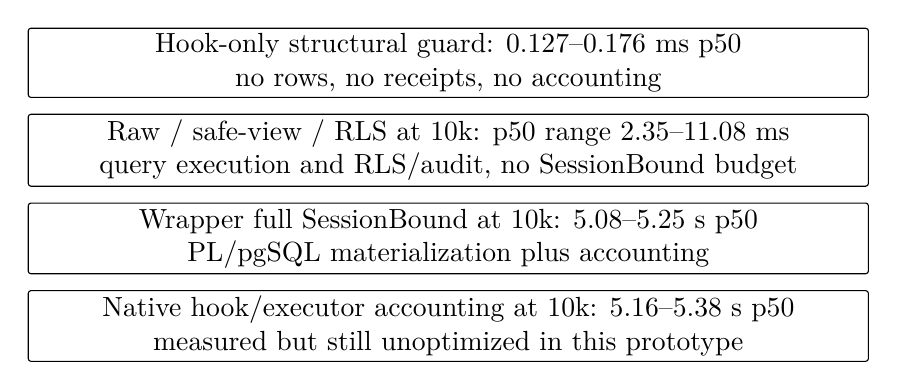
\begin{tikzpicture}[
  node distance=2mm,
  box/.style={draw, rounded corners=1pt, align=center, inner sep=2pt, minimum width=0.88\linewidth, minimum height=6mm}
]
\node[box] (h) {Hook-only structural guard: 0.127--0.176 ms p50\\no rows, no receipts, no accounting};
\node[box, below=of h] (b) {Raw / safe-view / RLS at 10k: p50 range 2.35--11.08 ms\\query execution and RLS/audit, no SessionBound budget};
\node[box, below=of b] (w) {Wrapper full SessionBound at 10k: 5.08--5.25 s p50\\PL/pgSQL materialization plus accounting};
\node[box, below=of w] (n) {Native hook/executor accounting at 10k: 5.16--5.38 s p50\\measured but still unoptimized in this prototype};
\end{tikzpicture}
\caption{Performance diagnosis. Structural guarding is sub-millisecond,
while both accounting-complete paths become multi-second at 10k rows;
the current bottleneck is result accounting/materialization rather than
parse/analyze checks.}
\label{fig:performance-diagnosis}
\end{figure}

The diagnostic native end-to-end benchmark in
Table~\ref{tab:scale-sweep} measures five query shapes over 1k and 10k
scoped rows using a bounded rerun with one warmup and three measured
iterations per shape. The SessionBound modes use API-issued runtime
credentials and signed task tokens, but API calls are outside measured
query latency. The wrapper mode executes through
\texttt{taskbound.run(sql)}. The native mode binds the same task token
and then issues direct safe-view SQL through the PostgreSQL hook and
executor-accounting path.

The result is intentionally conservative. Safe-view-only and
RLS+safe-view+audit baselines remain within roughly 12 ms p99 at 10k
rows across these query shapes. Both current SessionBound accounting
paths are much slower: wrapper p50 is 5.08--5.25 s and native
hook/executor p50 is 5.16--5.38 s at 10k rows. Thus the hook-only
structural result should not be presented as full SessionBound
performance. The current native accounting path demonstrates direct DB
enforcement semantics but has not yet delivered optimized scale
behavior.

The 10k-row setting intentionally raises the disclosure budget to
stress-test accounting completeness for larger detail releases. It
should not be interpreted as the common operating mode for approved
analytical tasks, where detail-release budgets are typically smaller and
aggregate queries dominate. Enterprise audits may scan many rows without
releasing every detail row to an agent; production deployments should
optimize aggregate-heavy executor accounting and route high-cardinality
detail exports through controlled workflows. The roadmap is cached task
descriptors, executor accounting, \texttt{DestReceiver}/CustomScan-style
integration, aggregate-first accounting, and less PL/pgSQL
materialization. These optimizations target moving high-cardinality
native accounting from PL/pgSQL-style materialization toward
executor-local streaming overhead, with the engineering goal of reducing
10k-row detail-release accounting from multi-second latency to
sub-second latency on similar hardware; this target remains future work
rather than an evaluated claim.

\hypertarget{scale-and-concurrency}{%
\subsection{Scale and concurrency}\label{scale-and-concurrency}}

We separately tested credential-token and safe-view drift edge cases; the
updated prototype denied all tested cases: credential A with token B,
replaying a token with a second credential, same-session second active
binding, wrong token audience or actor, expired token, revoked task
state, registry and safe-view policy-version drift, view-definition hash
mismatch, and exposed-column hash mismatch. Drift denials require
re-approval before execution.

On the default seed (430 expenses, 240 employees, and 124 departments),
an API concurrency smoke test completed 1, 5, and 20 concurrent sessions
with zero failed sessions. At 20 concurrent sessions, query p50 was
82.896 ms and query p95 was 110.356 ms. This is an API-stack smoke test,
not a throughput-capacity claim.
The concurrent isolation script confirmed independent credentials,
budgets, and task-specific receipts for two active tasks, and denied
credential A with token B and same-backend double binding. In the
concurrent isolation run, two active tasks executed interleaved queries
with independent query-count, result-row, and conservative tuple counters;
over-budget denial in one task did not change the other task's remaining
budget or receipt chain.

The new global single-active binding evaluation specifically targets the
same-key multi-backend gap. In
\texttt{single\_active\_binding\_20260710\_030846.json}, two synchronized
backends and a 20-contender race each produced exactly one owner. A
1000-round synchronized race produced 1000 single-winner rounds, zero
dual-success rounds, zero zero-winner rounds, and zero unexpected
errors. Explicit unbind, socket-close recovery,
\texttt{pg\_terminate\_backend} recovery, rollback-independent binding,
live-owner non-eviction, PID-reuse protection, stale fence rejection,
lock/utility tamper blocking, budget continuity, receipt-chain
continuity, and different-key concurrency all passed. Binding latency
over the same run had p50 13.017 ms, p95 17.780 ms, and p99 26.234 ms.

\begin{table}[!t]
\centering
\scriptsize
\setlength{\tabcolsep}{3pt}
\caption{Global single-active binding evaluation for one exact
\((\texttt{task\_id},\texttt{token\_digest},\texttt{credential\_id})\)
key.}
\label{tab:global-single-active}
\begin{tabular}{@{}p{0.56\linewidth}p{0.34\linewidth}@{}}
\toprule
Case & Result \\
\midrule
2 backends, same key & exactly 1 owner, 1 denial \\
20 backends, same key & exactly 1 owner, 19 denials \\
1000 repeated races & 0 dual-success, 0 zero-owner \\
Explicit unbind & immediate reacquisition \\
Socket close & stale recovery succeeds \\
Backend termination & stale recovery succeeds \\
Live idle owner & never time-evicted \\
Old fence mutation & rejected; 2 fenced events \\
Budget after recovery & preserved at 2 output tuples \\
Receipt chain after recovery & verified \\
Different binding keys & concurrent success \\
\bottomrule
\end{tabular}
\end{table}

We also ran a synthetic scale sweep over 1k and 10k scoped expense rows.
Table~\ref{tab:scale-sweep} reports p50 ranges across
\texttt{SELECT}, \texttt{JOIN}, \texttt{GROUP BY}, CTE, and window
queries, along with the maximum p95 and p99 observed across those
patterns. All listed measurements completed with zero query errors.
The 10k target is a detail-release stress setting with elevated
budgets; these results expose a scale-sensitive limitation shared by the
current wrapper and native accounting implementations and should not be
read as a production-throughput claim.

\begin{table}[!t]
\centering
\scriptsize
\setlength{\tabcolsep}{3pt}
\caption{Diagnostic end-to-end scale benchmark in milliseconds. p50 is
the range across five query shapes; p95/p99 are maxima. The current
rerun uses one warmup plus three measured iterations per shape and uses
elevated disclosure budgets as a detail-release stress test, not the
expected common operating mode.}
\label{tab:scale-sweep}
\begin{tabular}{@{}llcrrr@{}}
\toprule
Rows & Mode & p50 range & max p95 & max p99 & Err. \\
\midrule
1k & Raw & 0.69--1.25 & 1.38 & 1.38 & 0 \\
1k & Safe view & 0.89--1.47 & 1.62 & 1.62 & 0 \\
1k & RLS+SV+Audit & 1.95--2.22 & 2.76 & 2.76 & 0 \\
1k & SB wrapper & 570.26--746.62 & 769.12 & 769.12 & 0 \\
1k & SB native & 582.10--731.06 & 811.33 & 811.33 & 0 \\
10k & Raw & 2.35--9.68 & 9.71 & 9.71 & 0 \\
10k & Safe view & 3.47--10.82 & 10.88 & 10.88 & 0 \\
10k & RLS+SV+Audit & 4.03--11.08 & 11.82 & 11.82 & 0 \\
10k & SB wrapper & 5077.19--5253.43 & 5306.57 & 5306.57 & 0 \\
10k & SB native & 5163.18--5383.24 & 5526.78 & 5526.78 & 0 \\
\bottomrule
\end{tabular}
\end{table}

\hypertarget{remaining-gaps}{%
\subsection{Discussion of remaining gaps}\label{remaining-gaps}}

Several gaps remain. The PostgreSQL hook path now includes native
executor accounting, but the disclosure unit is still demo-specific and
the native path is not optimized across broad production workloads.
Minimum-group policy mitigates direct small-group aggregate release, but
arbitrary semantic inference across multiple allowed answers remains out
of scope; the budget vector is operational and does not provide formal
differential privacy.

\hypertarget{related-work}{%
\section{Related Work}\label{related-work}}

SessionBound is a task-session contract, while prior systems are
identity-, policy-, product-, operation-, or audit-centered. RLS,
short-lived credentials, safe views, and audit logs implement pieces, but
do not bind row scope, credential identity, SQL surface, cumulative
budget, drift checks, and decision-bound receipts into one approved
database session.

ABAC/XACML, capability systems, purpose-aware access, OAuth,
authenticated delegation, and Zanzibar provide authorization,
delegation, or relationship checks~\cite{nist2019abac,oasis2013xacml,dennis1966programming,miller2003capability,agrawal2002hippocratic,byun2008purpose,rfc6749,south2025authenticateddelegation,pang2019zanzibar};
SessionBound addresses how the resulting SQL session is scoped,
budgeted, drift-checked, and audited.

PAuth authorizes service/tool operations implied by a
task~\cite{sharma2026pauth}; Data Product MCP governs data-product
discovery, access, and contract-aware querying~\cite{tonnarelli2026dataproductmcp,mcp2025specification}.
SessionBound is complementary: after approval or data-product selection,
it enforces the PostgreSQL execution contract. Prompt-injection work,
information-flow controls, RLS/VPD/DDS,
parser-mediated validation, auditing, inference control, and
differential privacy address adjacent
pieces~\cite{greshake2023indirect,liu2023promptinjection,owasp2025llm01,myers1997difc,costa2025ifcagents,postgresql2026rowsecurity,oracle2026vpd,oracle2026deepdatasecuritydocs,oracle2026deepdatasecuritybrief,boyd2004sqlrand,su2006essence,kleinberg2000auditing,adam1989securitycontrol,dwork2014algorithmic};
SessionBound composes them around a task-bound database session with
operational accounting, not formal DP.


\hypertarget{limitations}{%
\section{Limitations}\label{limitations}}

SessionBound is a research prototype and reference architecture, not a
formal SQL safety proof. It targets one PostgreSQL database; production
needs KMS/JWKS signing, credential lifecycle management, safe-view
migration review, external audit retention, WORM anchoring, and external
primary fencing for HA. The global active-binding protocol assumes one
trusted writable PostgreSQL primary and is not a distributed consensus
protocol; cross-cluster binding and database split brain are out of
scope.
Disclosure budgets are operational authority accounting, not
differential privacy or complete semantic inference control:
minimum-group policy mitigates direct small-group aggregate release, but
inference across allowed answers and high-risk payload aggregation remain
out of scope. Measurements cover microbenchmarks, ablations, concurrency
smoke tests, and diagnostic 1k/10k scale benchmarks, not optimized
broad production workloads. Federation, malicious DBAs, and compromised
hosts are out of scope.

\hypertarget{conclusion}{%
\section{Conclusion}\label{conclusion}}

SessionBound turns enterprise task approval into budgeted database
sessions for AI agents: ``The agent can try. The database decides.'' It
binds approval, credential identity, safe-view versioning, SQL surface,
budgets, and receipts into one contract. The prototype shows
sub-millisecond structural guarding and multi-second accounting-complete
10k-row stress paths; production work must optimize result accounting, backend
state caching, and PostgreSQL executor integration without weakening it.

{\scriptsize
\bibliographystyle{IEEEtran}
\bibliography{references}
}

\end{document}
